\documentclass[11pt]{article}
\usepackage[utf8]{inputenc}
\usepackage[T1]{fontenc}
\usepackage[margin=1in]{geometry}
\usepackage{amsmath,amssymb,amsthm}
\usepackage{booktabs}
\usepackage{graphicx}
\usepackage{caption}
\usepackage[colorlinks=true,linkcolor=blue,citecolor=blue,urlcolor=blue]{hyperref}
\graphicspath{{figures/}}

\title{\textbf{The Angular Observer as a Manifold Recognizer}\\[2pt]
\large Reading Emergent Geometry from Hypergraph Rewriting}
\author{Andrew H. Bond\\ San Jos\'e State University\\
\texttt{andrew.bond@sjsu.edu} \quad ORCID 0009-0003-2599-6158}
\date{Working draft --- v0.1}

\begin{document}
\maketitle

\begin{abstract}
If space is a discrete network evolving under local rewrite rules, physics
needs an instrument that zooms out: given only nodes and edges, decide whether
a macro-geometry has emerged, and if so, \emph{which one}. The companion paper
\cite{kta} established the measuring tape---the angular coordinate of the
commute-weighted low-mode Laplacian embedding preserves graph geodesics where
the raw embedding degenerates into local density. This paper turns the
measuring tape into a \emph{recognizer}: a battery of five instruments
(density irregularity, dimension consensus, angular fidelity with controls, a
shape battery of flat-embedding stress / sphere-fit residual / eccentricity
homogeneity, and a low-spectrum multiplet signature scored against
closed-manifold templates) that identifies the manifold behind a graph, or
reports that there is none. The battery validates on ground truth: a sampled
flat torus is classified as a flat torus and a sampled sphere as $S^2$, from
spectra and angular distances alone. Pointed at five Wolfram-model rewrite
rules, it returns graded, interpretable verdicts: no rule grows a closed
manifold (all are bounded patches with an edge, eccentricity spread
$0.39$--$0.65$ against $\approx0.10$ for the closed controls); one rule is a
cleanly recognizable flat 2D patch; one is, at the tested growth stage, an
almost perfect \emph{interval} (spectrum ratios $1,3.7,8.1,14.5$ against the
$1,4,9,16$ template); one is genuinely fractal ($d\approx1.4$); and one is a
$\approx3.4$-dimensional space matching no manifold template. Two findings are
new. First, under a growth sweep ($750$--$12{,}000$ rewrite events),
\emph{dimension emerges before shape}: a rule's measured dimensionality locks
in at the earliest stages and is stable throughout, while its finer symmetry
class (patch vs.\ sphere vs.\ torus) can keep wandering---dimensionality is
the robust emergent invariant. Second, on emergent substrates the
Coifman--Lafon $\alpha{=}1$ density correction \emph{lowers} angular fidelity
even as it improves sampled manifolds---on a graph with no latent manifold,
density is structure, not sampling noise.
\end{abstract}

\section{Introduction}\label{sec:intro}
In discrete-spacetime programs---causal sets, causal dynamical triangulations,
and the Wolfram model \cite{wolfram2020,gorard2020}---the universe is a graph
or hypergraph and continuum geometry is supposed to emerge at scale. That
supposition needs an instrument. To say a hypergraph ``is'' an emergent
2-manifold is to claim that some coarse-graining of its combinatorics
converges to the metric geometry of a surface; the claim is empty without a
way to compute the coarse-graining and check the convergence.

Spectral embeddings are the natural candidate instrument, and they carry a
known pathology that is fatal in exactly this setting: on large geometric
graphs the commute (resistance) distance degenerates to a function of local
degrees \cite{vonluxburg2014}, and rewrite rules---localized, uncoordinated
---produce precisely the irregular node densities that trigger the
degeneracy. The companion paper \cite{kta} showed that the degeneracy is
confined to the \emph{radial} coordinate of the embedding: row-normalization
(the Ng--Jordan--Weiss step \cite{ng2002}) deletes the density factor, and the
surviving \emph{angular} coordinate preserves graph geodesics---with a
conditional transfer theorem, an unconditional instance on the flat torus, and
rank fidelity flat in mode budget and graph size across substrate families.

That result is a measuring tape: it certifies that angular distances track
geodesics. This paper asks the next question. Given the tape, can we read off
\emph{which} geometry a rewrite rule grows---recover smooth, recognizable
manifolds where they exist, and detect the spaces that are something else
entirely? We assemble a recognition battery (\S\ref{sec:battery}), validate it
on manifolds with known ground truth (\S\ref{sec:controls}), and point it at
five Wolfram-model rules (\S\ref{sec:rules}). Two phenomena beyond
recognition emerge: the verdicts \emph{move} as substrates grow
(\S\ref{sec:growth}), and the standard density-correction of manifold
learning is the wrong move on emergent substrates (\S\ref{sec:alpha}).

\section{The recognition battery}\label{sec:battery}
Let $G$ be the clique-expanded graph of an evolved hypergraph (largest
component, cropped to $n\le2000$), $L_{\mathrm{sym}}$ its symmetric-normalized
Laplacian with eigenpairs $(\lambda_k,v_k)$. The angular embedding is the
row-normalized commute-weighted map
$\hat u_i=\Psi_i/\lVert\Psi_i\rVert$,
$\Psi_i=(v_k(i)/\sqrt{\lambda_k})_{k=1}^{m}$, $m=20$, exactly as in
\cite{kta}; angular distances are chordal, geodesics are hop distances on
$150$ anchors. The battery has five instruments.

\textbf{(1) Density irregularity.} The degree coefficient of variation
$\mathrm{CV}(k_i)$: the driver of commute degeneracy \cite{vonluxburg2014},
and the regime rewrite rules inhabit.

\textbf{(2) Dimension consensus.} Ball-growth, spectral (heat-trace), and
effective-rank estimators; their mean is the measured intrinsic dimension $d$
and their spread the manifold-grade criterion, as in \cite{kta}.

\textbf{(3) Fidelity with controls.} Spearman angle-$\rho$ between angular
distances and geodesics; magnitude-only $\rho$; an equal-size random-mode
control (must be $\approx0$); and the Coifman--Lafon $\alpha{=}1$
density-normalized angle \cite{coifman2006} for \S\ref{sec:alpha}.

\textbf{(4) Shape battery.} Three coordinate-free discriminators of the
angular geometry $D_{\mathrm{ang}}$ on the anchor set:
\emph{flat-stress}, the residual stress of the best rank-2 (and rank-3)
classical MDS of $D_{\mathrm{ang}}$---a flat patch embeds at low stress, a
closed or curved geometry cannot;
\emph{sphere fit}, the relative RMS radial residual of the best-fit sphere to
the 3D MDS configuration;
\emph{homogeneity}, the spread $(\max-\min)/\mathrm{mean}$ of anchor
eccentricities---closed homogeneous manifolds are narrow, bounded patches are
broad.

\textbf{(5) Multiplet signature.} The low-spectrum ratios
$\lambda_k/\lambda_1$, $k=1,\dots,8$, scored (RMS log-distance) against four
templates: flat 2-torus $(1,1,1,1,2,2,2,2)$, sphere $S^2$ $(1,1,1,3,3,3,3,3)$,
Neumann square patch $(1,1,2,4,4,5,5,8)$, and interval
$(1,4,9,16,\dots)$. Multiplicity structure is a fingerprint of symmetry and
topology that survives discretization; for random geometric graphs the low
normalized-Laplacian spectrum converges to the Laplace--Beltrami spectrum
\cite{garciatrillos2018,calder2022}, so the templates are the right asymptotic
targets.

\section{Validation on known manifolds}\label{sec:controls}
The battery must first recognize geometry we can check. On a flat 2-torus
random geometric graph ($n=2000$) and a sphere $S^2$ graph ($n=2000$):
the torus is classified \emph{flat 2-torus} (signature distance $0.20$ vs
$0.34$ for the sphere template) and the sphere is classified \emph{sphere}
($0.17$ vs $0.56$ for the torus template) with the smallest sphere-fit
residual of any substrate ($0.10$); both show the closed-manifold profile the
shape battery predicts---high flat-stress ($0.54$, $0.48$: neither flattens
into $\mathbb R^2$) and near-uniform eccentricities (spread $0.11$, $0.09$).
Angle-$\rho$ is $0.90$ and $0.96$; magnitude and random controls are
$\le0.04$. The instrument can tell a torus from a sphere from a patch using
spectra and angular distances alone.

\section{Five rules, five verdicts}\label{sec:rules}
We point the battery at the five hypergraph-rewrite rules of the companion
paper's manifold library (arity-3, grown to a 3000-edge budget, seed 1;
single-seed caveats in \S\ref{sec:limits}).

\begin{center}\small
\begin{tabular}{lrrrrrrl}
\toprule
rule & $n$ & deg CV & $d$ (spread) & angle-$\rho$ & stress$_2$ & ecc.\ spr. & verdict \\
\midrule
torus control  & 2000 & 0.25 & 1.93 (0.09) & 0.90 & 0.54 & 0.11 & flat 2-torus \\
sphere control & 2000 & 0.26 & 1.83 (0.12) & 0.96 & 0.48 & 0.09 & sphere $S^2$ \\
\midrule
R\_2D    &  501 & 0.30 & 1.06 (0.20) & 0.92 & 0.21 & 0.65 & interval (a curve) \\
R\_frac  & 2000 & 0.06 & 1.39 (0.08) & 0.89 & 0.33 & 0.65 & fractal filament web \\
evolved-2D & 2000 & \textbf{1.42} & 2.03 (0.31) & 0.73 & 0.43 & 0.55 & ragged 2D patch \\
R\_3D    &  501 & 0.08 & 2.06 (\textbf{0.05}) & 0.82 & 0.52 & 0.48 & clean flat 2D patch \\
R\_SR    & 2000 & 0.90 & 3.36 (0.28) & 0.55 & 0.49 & 0.39 & no template ($\approx$3.4D) \\
\bottomrule
\end{tabular}
\end{center}

Four readings. \textbf{(i) No rule grows a closed manifold.} Every emergent
substrate has eccentricity spread $0.39$--$0.65$ against $\approx0.10$ for the
closed controls: these are \emph{bounded patches grown outward from a seed},
geometry with an edge---as a finite rewriting history should produce.
\textbf{(ii) The recognizable cases are genuinely recognizable.} R\_3D is a
flat-ish 2D patch with the tightest dimension consensus in the table (spread
$0.05$) and a square-patch signature; R\_2D, at this growth budget, is
identified as an \emph{interval} with near-exact spectrum
($1,3.7,8.1,14.5,23.2$ against $1,4,9,16,25$; signature distance $0.076$).
\textbf{(iii) The unexpected spaces are flagged, not force-fitted.} R\_frac is
genuinely fractal ($d\approx1.4$, filament clusters); R\_SR is a
$\approx3.4$-dimensional space whose spectrum matches no manifold template.
\textbf{(iv) Dimension gating shows up cross-substrate.} The two quasi-1D
rules have the highest magnitude-$\rho$ ($0.26$, $0.47$): the radius stays
geodesic-informative exactly where the radial-degeneracy corollary of
\cite{kta} does not apply. Random-mode controls are $\le0.02$ everywhere.

\begin{figure}[t]
\centering
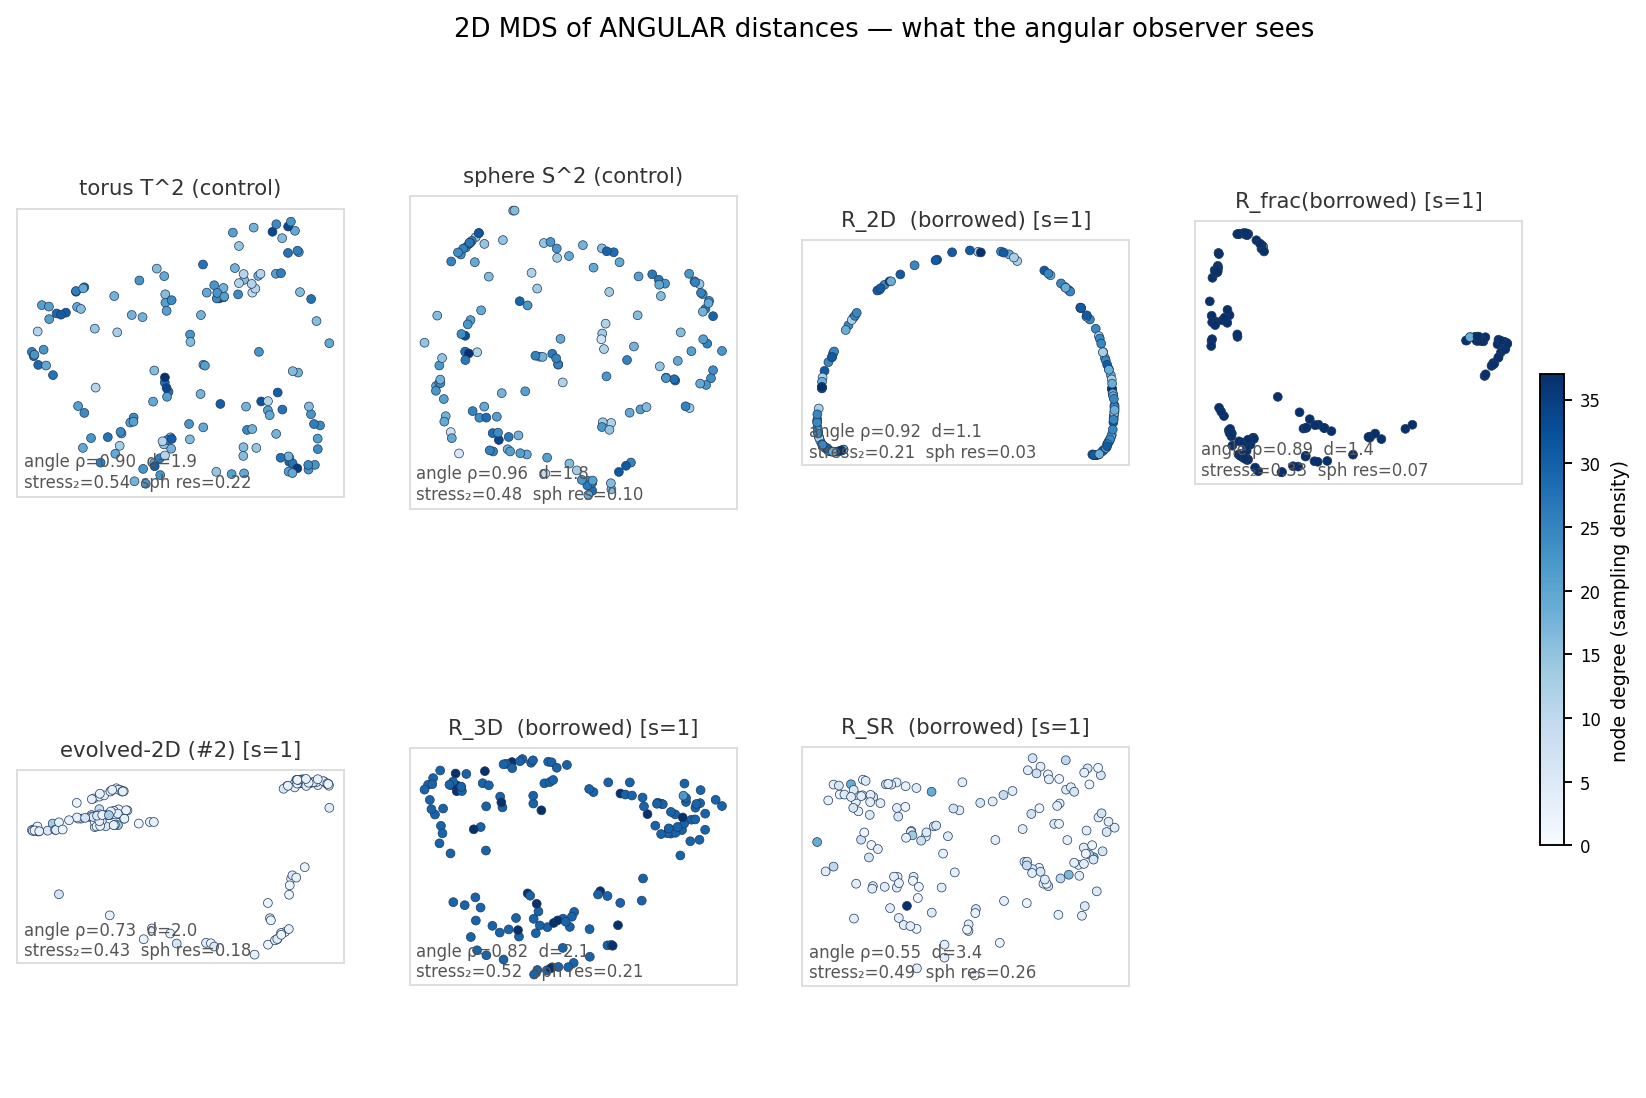
\includegraphics[width=\linewidth]{angular_layouts.png}
\caption{What the angular observer sees: 2D MDS of the \emph{angular}
distance matrix per substrate, points shaded by node degree (sampling
density). The closed controls fill the plane (they cannot be flattened); R\_2D
collapses onto a curve; R\_3D and evolved-2D are bounded 2D patches; R\_SR is
a diffuse high-dimensional cloud.}
\label{fig:layouts}
\end{figure}

\begin{figure}[t]
\centering
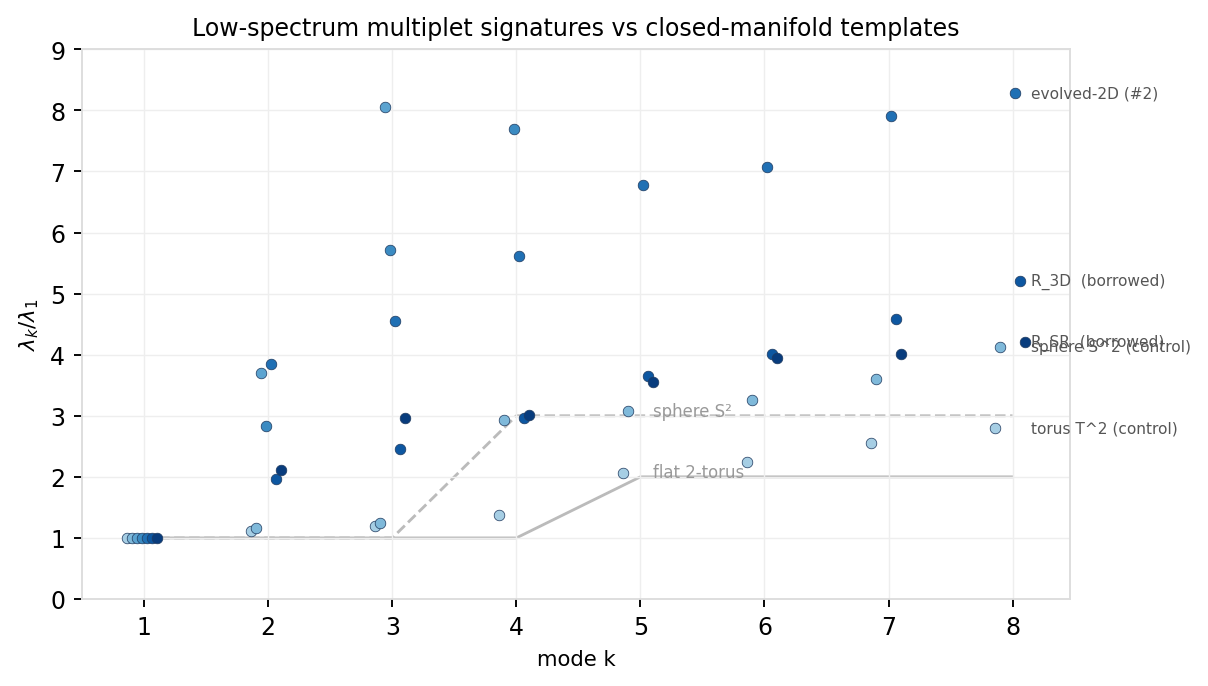
\includegraphics[width=0.85\linewidth]{spectral_signatures.png}
\caption{Low-spectrum multiplet signatures $\lambda_k/\lambda_1$ against
closed-manifold templates. The controls hug their templates (torus the solid
line, sphere the dashed); the emergent rules climb far faster---no
multiplet structure, hence no closed symmetry---which is exactly how the
battery separates patches and non-manifolds from closed geometry.}
\label{fig:signatures}
\end{figure}

\section{Dimension emerges before shape}\label{sec:growth}
Is ``R\_2D is a curve'' a fact about the rule or about the growth stage? We
sweep the rewrite budget over $750$--$12{,}000$ edges (generation cap scaled
with the budget; beyond $3000$ edges the recognizer reads a fixed 2000-node
geodesic-ball window of the larger substrate, i.e.\ a bounded observer probing
a growing universe) and re-run the recognizer at each stage
(Fig.~\ref{fig:growth}). Three growth behaviours appear, none the naive
``template crossing'' one might expect:

\textbf{R\_2D is a curve, definitively.} The interval signature is pinned at
distance $0.02$--$0.05$ at \emph{every} stage, with $d=1.04$--$1.06$ and
angle-$\rho=0.93$--$0.95$ throughout; the interior of the large substrate is
as one-dimensional as its early stages. The verdict of \S\ref{sec:rules} was
about the rule, not the stage.

\textbf{evolved-2D is a stable patch.} Square-patch wins at all five budgets
($d=1.94$--$2.05$): a robust, reproducible-under-growth identity.

\textbf{R\_3D: dimension locks first, shape does not.} The measured dimension
sits at $d\approx1.9$--$2.2$ from the earliest stage, and all three 2D
templates score in a tight band ($0.24$--$0.68$) far below interval
($1.85$--$2.32$)---but the \emph{winning} 2D template wanders: square patch
($750$) $\to$ sphere ($1500$) $\to$ flat torus ($3000$) $\to$ sphere ($6000$)
$\to$ square patch ($12{,}000$). The refined claim this supports:
\emph{dimensionality is the robust emergent invariant; symmetry class is
not}---at these scales R\_3D is unambiguously a 2D geometry that is not yet
(or not ever) any of the clean model spaces. Its angular fidelity also dips
and recovers across the sweep ($0.80\to0.59\to0.73$), consistent with the
fixed-budget observer effect documented in the companion paper's continuum
section: a fixed $m=20$ window resolves a shrinking fraction of a growing
substrate.

\begin{figure}[t]
\centering
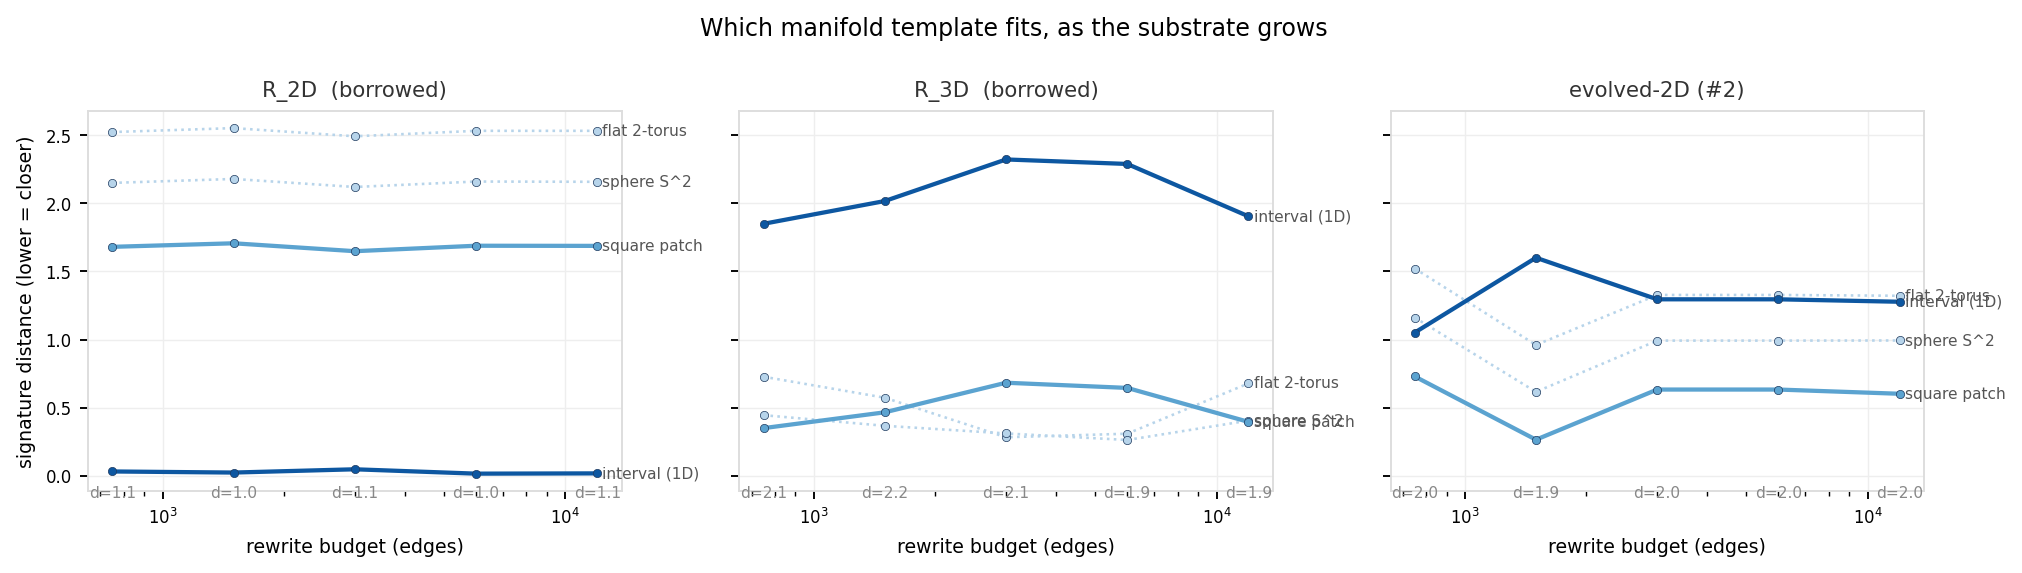
\includegraphics[width=\linewidth]{growth_signatures.png}
\caption{Which manifold template fits, as the substrate grows: multiplet
signature distance per template (lower = closer) across rewrite budgets,
measured dimension annotated per stage. R\_2D (left) is an interval at every
stage; evolved-2D (right) is a stable square patch; R\_3D (middle) locks its
\emph{dimension} at $\approx2$ immediately while the winning 2D template
wanders---dimension emerges before shape.}
\label{fig:growth}
\end{figure}

\section{Density is structure: the $\alpha{=}1$ dissociation}\label{sec:alpha}
On sampled manifolds, non-uniform node density is \emph{sampling noise}: the
graph Laplacian converges to a density-weighted operator, and the
Coifman--Lafon $\alpha{=}1$ normalization removes the weight, demonstrably
restoring angular fidelity under strong contrast \cite{coifman2006,kta}. The
recognizer reproduces that on the controls ($S^2$: $0.96\to0.98$; torus:
$0.90\to0.91$). On the emergent substrates the same correction moves fidelity
the \emph{other way}: evolved-2D $0.73\to0.64$, R\_3D $0.82\to0.81$, R\_SR
$0.55\to0.51$---mildly but consistently down, and most where degree CV is
largest. The reading: on a graph with no latent manifold underneath, the
density profile is not noise over a ground truth---it \emph{is} part of the
substrate's structure, and dividing it out removes signal. This gives the
density coordinate an unexpected second life: for sampled geometry it is a
nuisance parameter, for emergent geometry it is data, and the sign of the
$\alpha{=}1$ response is itself a diagnostic for which situation one is in.

\section{Limitations and falsifiers}\label{sec:limits}
Single seed per rule at each budget (the companion paper's library shows
seed-to-seed dimension variation, so per-rule verdicts should be read per
instance); hop-count geodesics; $n\le2000$ dense-eigensolver scale; four
templates, so ``matches none'' means none-of-these---hyperbolic, higher-genus,
and product templates are the obvious extensions; the growth sweep is a
budget sweep, not a fixed-rule time series at scale. Each is mechanical to
lift, none is conceptual. The recognizer is falsifiable in use: it must keep
classifying held-out sampled manifolds correctly (cylinders, genus-2
surfaces, $T^3$), and its emergent-substrate verdicts must be stable under
seeds and reproduce under budget for the claims here to stand.

\section{Outlook}\label{sec:disc}
The bridge claim, stated with its bounds: for a universe built purely of
nodes and edges, the angular coordinate of the low-mode spectral embedding is
a mathematically controlled zoom-out---the companion paper supplies the
guarantees, and this paper shows the zoom-out is \emph{legible}: it does not
merely score geodesic fidelity, it reads off dimension, boundedness,
curvature class, and symmetry, and it declines to hallucinate a manifold
where none exists. In observer-theoretic terms \cite{wolfram2026}, the
recognizer is a concrete, falsifiable candidate for the coarse-graining a
bounded observer performs; nothing here requires that reading, and the
strongest physics-adjacent findings---bounded patches rather than closed
universes, dimension arriving under growth, density as structure---stand as
graph-theoretic facts about rewrite systems.

\paragraph{Reproducibility.} \texttt{experiments/manifold-recovery/} in the
companion repository
(\url{https://github.com/ahb-sjsu/the-angular-observer}) contains the
recognizer (\texttt{recover.py}), the growth sweep
(\texttt{growth\_sweep.py}), committed result JSONs, and the figure scripts;
all runs are seeded, CPU-only, NumPy/SciPy.

\begin{thebibliography}{9}
\bibitem{kta} A.~H.~Bond. Keep the angle: a geometry-preserving basis in
spectral embeddings. Working draft v0.8,
\url{https://github.com/ahb-sjsu/the-angular-observer}, 2026.
\bibitem{vonluxburg2014} U.~von~Luxburg, A.~Radl, and M.~Hein. Hitting and
commute times in large random neighborhood graphs. \emph{JMLR},
15:1751--1798, 2014.
\bibitem{ng2002} A.~Ng, M.~Jordan, and Y.~Weiss. On spectral clustering:
analysis and an algorithm. \emph{NeurIPS 14}, 2002.
\bibitem{coifman2006} R.~Coifman and S.~Lafon. Diffusion maps. \emph{Applied
and Computational Harmonic Analysis}, 21(1):5--30, 2006.
\bibitem{garciatrillos2018} N.~Garc\'ia Trillos and D.~Slep\v{c}ev. A
variational approach to the consistency of spectral clustering. \emph{Applied
and Computational Harmonic Analysis}, 45(2):239--281, 2018.
\bibitem{calder2022} J.~Calder and N.~Garc\'ia Trillos. Improved spectral
convergence rates for graph Laplacians on $\varepsilon$-graphs and $k$-NN
graphs. \emph{Applied and Computational Harmonic Analysis}, 60:123--175, 2022.
\bibitem{wolfram2020} S.~Wolfram. Finally we may have a path to the
fundamental theory of physics\ldots and it's beautiful. Writings blog, April
2020.
\bibitem{gorard2020} J.~Gorard. Some relativistic and gravitational properties
of the Wolfram model. \emph{Complex Systems}, 29(2):107--192, 2020.
\bibitem{wolfram2026} S.~Wolfram. The concept of the ruliad. Writings blog,
November 2021.
\end{thebibliography}

\end{document}
